% =============================================================================
\bloco{2}{Policy: optimal rules, the zero bound and household debt}{Benigno \S\S6--12 \,\textbullet\, 25 points}

\questao{(10 points) Objective items. Ranges: $\sigma,\eta,\kappa,\Delta>0$; the long run is unchanged unless stated.}

\textbf{a)} (3 points) \emph{Monetary $\times$ fiscal policy.} A temporary cut $\Delta$ in the consumption tax (like the 2009 IPI cut on
cars: $\tau_c=-\Delta$, $\bar\tau_c=0$), entering the markup one for one, changes natural output $y_n$ and the natural real rate
$r_n$ (the rate at which demand equals $y_n$) by, respectively:
\begin{alternativas}
\item $\left(\frac{\Delta}{\sigma^{-1}+\eta},\ \frac{\eta\,\Delta}{\sigma^{-1}+\eta}\right)$
\item $\left(\frac{\Delta}{\sigma^{-1}+\eta},\ -\frac{\sigma^{-1}\Delta}{\sigma^{-1}+\eta}\right)$
\item $\left(\frac{(1+\eta)\Delta}{\sigma^{-1}+\eta},\ \frac{(1-\sigma^{-1})\eta\,\Delta}{\sigma^{-1}+\eta}\right)$
\item $\left(\frac{\Delta}{\sigma^{-1}+\eta},\ \frac{(2\sigma^{-1}+\eta)\Delta}{\sigma^{-1}+\eta}\right)$
\end{alternativas}
\gabarito{A}
\begin{sol}
\passo{supply channel}{By (13) the markup falls by $\Delta$, so by (15), $y_n=\frac{(1+\eta)a+\sigma^{-1}g-\mu}{\sigma^{-1}+\eta}$ rises by $\frac{\Delta}{\sigma^{-1}+\eta}$; $\bar y_n$
stays (the cut is temporary), so the term $\sigma^{-1}(\bar y_n-y_n)$ of $r_n$ falls by $\frac{\sigma^{-1}\Delta}{\sigma^{-1}+\eta}$.}
\passo{demand channel}{Taxed consumption enters the Euler equation, $\bar c-c=\tilde\sigma[i-(\bar p-p)-(\bar\tau_c-\tau_c)-\rho]$, and so the AD
(21); setting $y=y_n$, $r_n=\rho+\sigma^{-1}(\bar y_n-y_n)+\sigma^{-1}(g-\bar g)+(\bar\tau_c-\tau_c)$. Consumption is cheaper today than tomorrow: the
last term of $r_n$ rises by $\Delta$.}
\passo{net}{$\Delta r_n=\Delta-\frac{\sigma^{-1}\Delta}{\sigma^{-1}+\eta}=\frac{\eta\Delta}{\sigma^{-1}+\eta}>0$, zero only if $\eta=0$: demand wins, so keeping $y=y_n$ needs a
slightly higher $i$. B keeps the supply channel only (the tax treated as a payroll tax); C reads the markup cut as a
productivity gain (coefficient $1+\eta$ in (15)); D flips the sign of the supply channel (a higher current $y_n$ read as raising $r_n$).}
\refbib{Benigno (2015), \S4.1, eqs.\ (13) and (15); \S5, eq.\ (21); \S8.}
\end{sol}

\medskip
\textbf{b)} (3 points) \emph{Fiscal multipliers.} Let $\Omega\equiv(\sigma^{-1}+\eta)(1+\sigma\kappa)$. With $i$, $\bar p$ and $p^e$ fixed, a temporary
rise in $g$ ($\bar g$ unchanged, lump-sum financed) changes output and the gap $y-y_n$, per unit of $g$, by:
\begin{alternativas}
\item $\left(\frac{\sigma^{-1}+\eta}{\Omega},\ \frac{\sigma^{-1}+\eta}{\Omega}\right)$
\item $\left(\frac{\sigma^{-1}+\eta+\kappa}{\Omega},\ \frac{\sigma^{-1}+\eta+\kappa}{\Omega}\right)$
\item $\left(\frac{\sigma^{-1}+\kappa}{\Omega},\ 0\right)$
\item $\left(\frac{\sigma^{-1}+\eta+\kappa}{\Omega},\ \frac{\eta}{\Omega}\right)$
\end{alternativas}
\gabarito{D}
\begin{sol}
\passo{both curves move}{The AD (21) shifts right by $dg$ and, by (15), the AS by $dy_n=\frac{\sigma^{-1}}{\sigma^{-1}+\eta}dg$. Substituting the AS into
the AD, $(1+\sigma\kappa)\,dy=dg+\sigma\kappa\,dy_n$, so $\frac{dy}{dg}=\frac{1}{1+\sigma\kappa}+\frac{\kappa}{\Omega}=\frac{\sigma^{-1}+\eta+\kappa}{\Omega}$.}
\passo{gap}{$\frac{d(y-y_n)}{dg}=\frac{\sigma^{-1}+\eta+\kappa-\sigma^{-1}(1+\sigma\kappa)}{\Omega}=\frac{\eta}{\Omega}>0$ (zero if $\eta=0$: the curves shift in proportion), and
$\frac{dy}{dg}-1=-\frac{\sigma\eta\kappa}{\Omega}<0$. A forgets the AS shift (pure demand); B measures the gap from the old $y_n$; C uses flexible
prices (output jumps to the new $y_n$).}
\refbib{Benigno (2015), \S8, eqs.\ (22)--(23), Table 1.}
\end{sol}

\medskip
\textbf{c)} (2 points, T or F) At the zero lower bound with $r_n<0$, a credible commitment to a long-run price level higher by
$-r_n$ restores $y=y_n$ and $p=p^e$, and the size of the commitment needed does not depend on the degree of price rigidity.
\gabarito{T}
\begin{sol}
\passo{proof}{Substituting the AS into the AD, $y-y_n=\frac{\sigma}{1+\sigma\kappa}[r_n-i+(\bar p-p^e)]$; at $i=0$ it vanishes iff $\bar p-p^e=-r_n$, for
every $\kappa$, and then $p=p^e$ by the AS. And nothing in $r_n$ ($\rho$, $\sigma$, fiscal terms, the flexible-price outputs $y_n,\bar y_n$)
involves $\alpha$: rigidity scales the slump, not the cure.}
\refbib{Benigno (2015), \S9.}
\end{sol}

\medskip
\textbf{d)} (2 points, T or F) \emph{AS--AD $\times$ household debt.} In the borrower--saver economy of Question 4(d), with constant
inflation between the short and the long run, more price flexibility reduces the output cost of a deleveraging shock.
\gabarito{F}
\begin{sol}
\passo{paradox of flexibility}{With $\bar p_n-p$ fixed, only the Fisher term of (32) moves with $p$: $\frac{dy}{dp}=\frac{(1-\chi)d_0}{\chi}>0$. With the AS and
$y_n$ unchanged, from a zero gap $y=\frac{(1-\chi)\hat d}{\chi-(1-\chi)d_0\kappa}$ and $\frac{\partial y}{\partial\kappa}=\frac{(1-\chi)^2d_0\,\hat d}{[\chi-(1-\chi)d_0\kappa]^2}<0$ for $\hat d<0$: the fall
grows with $\kappa$ on the whole stable range (Question 4(e)).}
\refbib{Benigno (2015), \S10, eq.\ (32).}
\end{sol}

% -----------------------------------------------------------------------------
\questao{(15 points) Discursive. \emph{Optimal policy $\times$ zero lower bound $\times$ household debt.} Ranges: $\sigma,\kappa,\rho>0$,
$\eta\ge0$, $\theta>1$; in (d)--(e), $\chi\in(0,1)$, $d_0>0$, $\beta\in(0,1)$. Shocks are temporary.}

\textbf{a)} (3 points) The bank minimizes Benigno's welfare loss $L=\tfrac12(y-y_e)^2+\tfrac{\theta}{2\kappa}(p-p^e)^2$ (eq.\ 33) subject to the AS.
Find the optimal relation between the efficient gap and price surprises, describe it in the $(y,p)$ plane, and prove that
shocks that leave $\mu$ unchanged create no trade-off.
\resolespaco
\begin{sol}
\passo{substitution}{The bank picks $y$ by moving $i$ along the AD, and the AS ties $p-p^e=\kappa(y-y_n)$ to it:
$L(y)=\tfrac12(y-y_e)^2+\tfrac12\theta\kappa(y-y_n)^2$, with $L''=1+\theta\kappa>0$, so the FOC gives the unique minimum.}
\passo{targeting rule}{FOC: $(y-y_e)+\theta\kappa(y-y_n)=0$, i.e.\ $(y-y_e)+\theta(p-p^e)=0$ (eq.\ 34), so $y^*=\frac{y_e+\theta\kappa y_n}{1+\theta\kappa}$, a weighted
average of the targets. In the $(y,p)$ plane the rule is the line through $(y_e,p^e)$ with slope $-1/\theta$; the optimum is where
it meets the AS (slope $\kappa$, through $(y_n,p^e)$).}
\passo{no trade-off}{By (15) and (19), $y_n-y_e=-\frac{\mu}{\sigma^{-1}+\eta}$. If $\mu$ does not move ($\mu=0$ around the efficient steady state),
$y_n=y_e$ and $(y_e,p^e)$ lies on both lines with $L=0$, the global minimum (divine coincidence), reached with $i=r_n+(\bar p-p^e)$,
which zeroes $y-y_n=\frac{\sigma}{1+\sigma\kappa}[r_n-i+(\bar p-p^e)]$.}
\intuicao{Welfare wants output at $y_e$, pricing ties prices to $y-y_n$; the bank trades the two gaps at the rate $\theta\kappa$, and
only a markup shock pulls the targets apart.}
\refbib{Benigno (2015), \S11, eqs.\ (33)--(34); \S4.4, eq.\ (19).}
\rubrica{
\item Substitution, FOC and second-order condition: 1.5 pts. Rule quoted: item max.\ 1 pt.
\item Geometry of the rule: 0.5 pt.
\item No trade-off proved from $y_n-y_e$: 1 pt; asserted without it: 0.
}
\end{sol}

\textbf{b)} (3 points) A temporary cost-push shock raises the markup by $\mu>0$ and moves productivity by $a$ (either sign;
Question 2(d) is the case $a<0$); $\bar y_n=0$, $\bar p=p^e$, $g=\bar g$. Find the optimal $y$, $p-p^e$ and $i$; compare them and the loss with
strict price stability; say which part of the shock $i$ offsets one for one. Show that no Taylor rule $i=\bar\imath+\psi_y(y-y_e)+\psi_\pi(p-p^e)$,
$\psi_y,\psi_\pi\ge0$, with a constant intercept $\bar\imath$ (a policy constant, not a long-run value) implements the optimum under all
productivity shocks.
\resolespaco
\begin{sol}
\passo{optimum}{With $M\equiv\frac{\mu}{\sigma^{-1}+\eta}=y_e-y_n$, (a) gives $y^*-y_n=\frac{M}{1+\theta\kappa}>0$, $y^*-y_e=-\frac{\theta\kappa M}{1+\theta\kappa}<0$, $p-p^e=\frac{\kappa M}{1+\theta\kappa}>0$,
between the pure policies ($-M$ and $\kappa M$). Strict price stability ($y=y_n$, $p=p^e$) costs $L^{PS}=\tfrac12M^2$; the optimum,
$L^*=\tfrac12\frac{\theta\kappa}{1+\theta\kappa}M^2$, so $L^*/L^{PS}=\frac{\theta\kappa}{1+\theta\kappa}<1$.}
\passo{interest rate}{By the gap formula with $\bar p=p^e$, $i^*=r_n-\frac{(\sigma^{-1}+\kappa)M}{1+\theta\kappa}<r_n$, the strict-price-stability rate, where
$r_n=\rho+\frac{\sigma^{-1}[\mu-(1+\eta)a]}{\sigma^{-1}+\eta}$. The productivity part moves $y_n$ and $y_e$ equally and reaches $i^*$ only through $r_n$: it is
offset one for one. Against the passive $i=\rho$: $i^*-\rho=\frac{\kappa(\theta\sigma^{-1}-1)\mu-\sigma^{-1}(1+\eta)(1+\theta\kappa)a}{(\sigma^{-1}+\eta)(1+\theta\kappa)}$, positive if $a\le0$ and
$\theta>\sigma$; with $a=0$ the bank eases iff $\theta<\sigma$.}
\passo{Taylor rule}{With $\mu=0$, $y_n=y_e$, the rule is $i=\bar\imath+(\psi_y+\psi_\pi\kappa)(y-y_n)$ and the gap formula gives
$y-y_n=\frac{r_n-\bar\imath}{\sigma^{-1}+\kappa+\psi_y+\psi_\pi\kappa}$: the optimum needs $\bar\imath=r_n$, yet $\frac{\partial r_n}{\partial a}=-\frac{\sigma^{-1}(1+\eta)}{\sigma^{-1}+\eta}\neq0$: a fixed intercept fits
one $a$ at most, and feedback only shrinks the error (to zero as $\psi_\pi\to\infty$).}
\intuicao{A cost-push shock is shared between output and prices as $\theta\kappa:1$; a productivity shock needs no sharing,
only an $i$ that follows $r_n$.}
\refbib{Benigno (2015), \S11.}
\rubrica{
\item Optimal $y$, $p$ and the loss ratio: 1 pt.
\item Optimal $i$, one-for-one offset, sign condition: 1 pt; a sign without the closed form: 0.
\item Taylor-rule argument with the gap under the rule: 1 pt.
}
\end{sol}

\textbf{c)} (3 points) Pessimism: long-run productivity is expected to fall, $\bar a<0$, with $a=\mu=0$ and $g=\bar g$. Find when the zero
bound binds, the outcome at $i=0$ with $\bar p=p^e$, and the $\bar p$ that restores the optimum; give the limits as $\kappa\to\infty$ and
$\kappa\to0$, and discuss credibility.
\resolespaco
\begin{sol}
\passo{natural rate}{By (15) with bars, $\bar y_n=\frac{(1+\eta)\bar a}{\sigma^{-1}+\eta}<0$, while $y_n=y_e=0$: $r_n=\rho+\sigma^{-1}\bar y_n=\rho+\frac{(1+\eta)\bar a}{1+\sigma\eta}$. With $\mu=0$
there is no trade-off and the optimum $y=0$, $p=p^e$ needs $i=r_n$, which the bound forbids iff $r_n<0$, i.e.\
$\bar a<-\frac{\rho(1+\sigma\eta)}{1+\eta}$: pessimism must outweigh impatience.}
\passo{at $i=0$}{The gap $\frac{\sigma(r_n-i)}{1+\sigma\kappa}$ is negative and closest to zero at $i=0$: $y=\frac{\sigma r_n}{1+\sigma\kappa}<0$, $p-p^e=\frac{\sigma\kappa r_n}{1+\sigma\kappa}<0$, a slump with
deflation. The bound caps the nominal rate, not the real one: $\bar p-p^e=-r_n>0$ zeroes $r_n+(\bar p-p^e)$, so $y=0$, $p=p^e$ at $i=0$.}
\passo{limits and credibility}{As $\kappa\to\infty$, $\frac{\sigma\kappa}{1+\sigma\kappa}\to1$: $y\to0$, $p-p^e\to r_n$ (prices absorb the shock); as $\kappa\to0$, $p\to p^e$ and
$y\to\sigma r_n$ (output does). Once the slump is over, a price-stability bank would rather set $\bar p=p^e$: the promise is
time-inconsistent and works only if believed.}
\intuicao{Pessimism makes households want to save; only a negative real rate clears that wish, and at $i=0$ it must come
from expected inflation, which the bank can only promise.}
\refbib{Benigno (2015), \S6.3 and \S9.}
\rubrica{
\item $r_n$ and the binding condition: 1 pt.
\item Outcome at $i=0$ and the required $\bar p$: 1 pt.
\item Limits from the closed forms, and credibility: 1 pt; limits without the closed form: 0.
}
\end{sol}

\textbf{d)} (3 points) With borrowers and savers (share $\chi$ of savers, initial debt $d_0$), Benigno's AD is
\[y=\bar y_n-\varphi[i-(\bar p_n-p)-\rho]+\tfrac1\chi(g-\bar g)+\tfrac{1-\chi}{\chi}[\hat d+d_0(p-p^e)],\qquad\varphi\equiv\frac{\sigma\chi+(1-\chi)d_0\beta}{\chi},\]
where $\bar p_n$ is the long-run price level ($\bar p$ above) and $\hat d$ the change in the debt limit. Find $dy/dp$ when $\bar p_n$ is anchored and when inflation $\bar p_n-p$ is constant,
naming the two channels. Assuming the anchored AD slopes down and, under constant inflation, the AD is steeper than the AS,
derive the spending multipliers $m_A$, $m_C$ ($i$ fixed), order them against $1/\chi$, and find when $m_A>1$.
\resolespaco
\begin{sol}
\passo{slopes}{Anchored: $\frac{dy}{dp}=-\varphi+\frac{(1-\chi)d_0}{\chi}=-\varpi$, $\varpi\equiv\sigma-\frac{d_0(1-\beta)(1-\chi)}{\chi}$. Real-rate channel: a higher $p$ lowers expected
inflation and raises the real rate, cutting savers' consumption ($-\sigma$) and what borrowers may borrow ($-\frac{(1-\chi)d_0\beta}{\chi}$). Fisher
channel: it erodes inherited nominal debt ($+\frac{(1-\chi)d_0}{\chi}$). As $\beta<1$, $\varpi<\sigma$: debt steepens the AD, which slopes down iff
$\varpi>0$. Constant inflation: the real rate no longer moves with $p$, and $\frac{dy}{dp}=\frac{(1-\chi)d_0}{\chi}>0$.}
\passo{multipliers}{A temporary $g$ shifts the AD by $\frac{dg}{\chi}$ and, by (15), raises $y_n$ by $s\,dg$, $s\equiv\frac{1}{1+\sigma\eta}\le1$; the AS gives
$dp=\kappa(dy-s\,dg)$. Anchored: $dy=\frac{dg}{\chi}-\varpi\kappa(dy-s\,dg)$, so $m_A=\frac{1/\chi+\varpi\kappa s}{1+\varpi\kappa}$. Constant inflation, with $x\equiv(1-\chi)d_0\kappa$:
$\chi\,dy=dg+x(dy-s\,dg)$, so $m_C=\frac{1-xs}{\chi-x}$, for $x<\chi$ (AD steeper than AS).}
\passo{ordering}{$m_A$ averages $\frac1\chi$ and $s<\frac1\chi$ with weight $\frac{\varpi\kappa}{1+\varpi\kappa}\in(0,1)$ on $s$, so $s<m_A<\frac1\chi$; and $m_C-\frac1\chi=\frac{x(1-\chi s)}{\chi(\chi-x)}>0$:
$m_C>\frac1\chi>m_A$. Next, $m_A>1$ iff $\varpi\kappa(1-s)<\frac{1-\chi}{\chi}$, i.e.\ $\varpi\kappa<\frac{(1-\chi)(1+\sigma\eta)}{\chi\sigma\eta}$ (always if $\eta=0$), while
$m_C-1=\frac{(1-\chi)+x(1-s)}{\chi-x}>0$. As $\chi\to1$, $\varpi\to\sigma$ and $m_A\to\frac{1+\sigma\kappa s}{1+\sigma\kappa}=\frac{\sigma^{-1}+\eta+\kappa}{\Omega}$, the multiplier of Question 3(b).}
\intuicao{Borrowers spend current income: the AD holds a Keynesian cross with multiplier $1/\chi$. Spending raises prices;
with $\bar p_n$ anchored that raises the real rate and crowds out ($m_A<1/\chi$), with constant inflation it only deflates real
debt and adds demand ($m_C>1/\chi$).}
\refbib{Benigno (2015), \S10, eq.\ (32) and footnote 19.}
\rubrica{
\item Both slopes with the two channels: 1 pt.
\item Both multipliers derived: 1 pt (quoted: item max.\ 1 pt; \S8 multiplier used: item max.\ 1.5 pts).
\item Ordering and the condition for $m_A>1$, proved: 1 pt.
}
\end{sol}

\textbf{e)} (3 points) \emph{Parameter analysis.} A deleveraging shock lowers the debt limit, $\hat d<0$, with $i$, $g$ fixed and the economy
initially at $y=y_n=0$, $p=p^e$. Find each regime's output response and the stability bound; sign both responses and
both multipliers of (d) against $\kappa$, $d_0$, $\chi$, $\sigma$ (given $\kappa$) in a table, with proofs; give the limits in $\kappa$ and the
knife-edges; draw both responses against $\kappa$ and read them.
\resolespaco
\begin{sol}
\passo{closed forms and bound}{$\hat d$ leaves $y_n$ unchanged (natural output does not depend on who holds the debt), so the AS is
$p-p^e=\kappa y$. Anchored: $y(1+\varpi\kappa)=\frac{1-\chi}{\chi}\hat d$, so $y_A=\frac{(1-\chi)\hat d}{\chi(1+\varpi\kappa)}$. Constant inflation: $\chi y=(1-\chi)(\hat d+d_0\kappa y)$, so
$y_C=\frac{(1-\chi)\hat d}{\chi-x}$, negative only for $\kappa<\kappa_{\max}\equiv\frac{\chi}{(1-\chi)d_0}$ and unbounded as $\kappa\uparrow\kappa_{\max}$: the stability bound, where the AD
slope in the $(y,p)$ plane, $\frac{\chi}{(1-\chi)d_0}$, equals the AS slope $\kappa$ (footnote 19).}
\passo{signs}{Let $\ell_j\equiv-y_j>0$. (i) $\ell_A$ falls with $\varpi\kappa$; $\varpi$ rises with $\sigma$ and falls with $d_0$; and
$\chi(1+\varpi\kappa)=\chi(1+\sigma\kappa)-(1-\beta)d_0(1-\chi)\kappa$ rises with $\chi$ while $1-\chi$ falls. (ii) $\frac{\partial\ell_C}{\partial\kappa}=\frac{(1-\chi)^2d_0|\hat d|}{(\chi-x)^2}>0$,
$\frac{\partial\ell_C}{\partial d_0}=\frac{(1-\chi)^2\kappa|\hat d|}{(\chi-x)^2}>0$, $\frac{\partial\ell_C}{\partial\chi}=-\frac{|\hat d|}{(\chi-x)^2}<0$; $\sigma$ is absent. (iii) $\frac{\partial m_A}{\partial(\varpi\kappa)}=\frac{s-1/\chi}{(1+\varpi\kappa)^2}<0$,
$\frac{\partial m_A}{\partial s}=\frac{\varpi\kappa}{1+\varpi\kappa}>0$, $\frac{\partial m_A}{\partial(1/\chi)}>0$, and $s$ falls with $\sigma$ (if $\eta>0$). (iv) By (d), $m_C$ rises with $x$ and,
as $\frac{\partial m_C}{\partial s}=-\frac{x}{\chi-x}<0$, falls with $s$; $\frac{\partial m_C}{\partial\chi}=-\frac{1+d_0\kappa(1-s)}{(\chi-x)^2}<0$.}
\par\smallskip\noindent
\begin{minipage}[c]{0.40\linewidth}
\centering
\begin{tabular}{lcccc}
\toprule
 & $\kappa$ & $d_0$ & $\chi$ & $\sigma$ \\
\midrule
$\ell_A$ & $-$ & $+$ & $-$ & $-$ \\
$\ell_C$ & $+$ & $+$ & $-$ & $0$ \\
$m_A$ & $-$ & $+$ & $-$ & $-$ \\
$m_C$ & $+$ & $+$ & $-$ & $+$ \\
\bottomrule
\end{tabular}
\par\smallskip{\footnotesize $\sigma$ at given $\kappa$; $\partial m_C/\partial\sigma=0$ if $\eta=0$.}
\end{minipage}\hfill
\begin{minipage}[c]{0.58\linewidth}
\centering
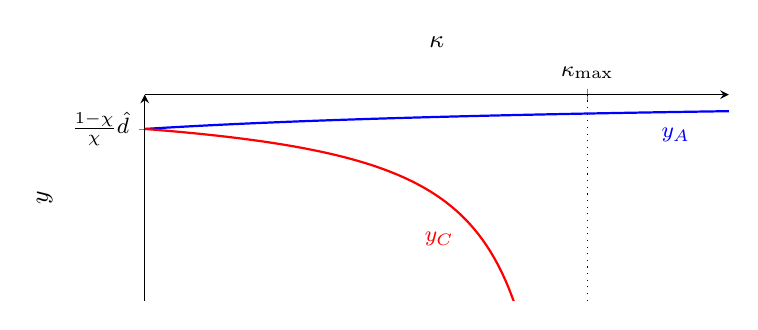
\begin{tikzpicture}
\begin{axis}[width=9cm,height=4.2cm,xmin=0,xmax=2.2,ymin=-0.3,ymax=0,axis x line=top,axis y line=left,
  xlabel={$\kappa$},ylabel={$y$},xtick={1.6667},xticklabels={$\kappa_{\max}$},ytick={-0.05},yticklabels={$\frac{1-\chi}{\chi}\hat d$},
  tick label style={font=\footnotesize},label style={font=\small}]
\addplot[thick,blue,domain=0:2.2,samples=80]{-0.05/(1+0.488*x)};
\addplot[thick,red,domain=0:1.6,samples=160]{(-0.1/3)/(2/3-0.4*x)};
\addplot[dotted] coordinates {(1.6667,-0.3) (1.6667,0)};
\node[font=\footnotesize,blue,anchor=north] at (axis cs:2.0,-0.035) {$y_A$};
\node[font=\footnotesize,red,anchor=east] at (axis cs:1.2,-0.21) {$y_C$};
\end{axis}
\end{tikzpicture}
\end{minipage}
\par\smallskip
\passo{limits}{$\kappa\to0$: $y_A,y_C\to\frac{1-\chi}{\chi}\hat d$ and $m_A,m_C\to\frac1\chi$ (prices do not move). $\kappa\to\infty$: $y_A\to0$, $m_A\to s$. $\kappa\uparrow\kappa_{\max}$:
$\ell_C,m_C\to\infty$. Knife-edges: $\chi\to1$ removes the debt channel ($y_A,y_C\to0$, $m_C\to1$); $\varpi=0$, i.e.\ $d_0=\frac{\sigma\chi}{(1-\beta)(1-\chi)}$, makes
the anchored AD vertical, so $y_A$ and $m_A=\frac1\chi$ do not depend on $\kappa$.}
\intuicao{With $\bar p_n$ anchored, a lower $p$ raises expected inflation and cuts the real rate: flexibility cushions the slump.
With constant inflation it lowers future prices too and raises real debt: flexibility deepens the slump (paradox of
flexibility). $\ell_C$ and $m_C$ share the denominator $\chi-x$: spending is most powerful where the slump is deepest.}
\refbib{Benigno (2015), \S10, eq.\ (32) and footnotes 19--20.}
\rubrica{
\item Closed forms and the stability bound: 1 pt.
\item Signs proved, limits, reading: 1 pt (signs unproved or unread: item max.\ 1.5 pts).
\item Graph, scored on its own: labels, common intercept, $y_A$ rising to 0, $y_C$ diverging at $\kappa_{\max}$: 1 pt.
}
\end{sol}
